\documentclass[czech,bachelor,dept460,male,csharp,cpdeclaration]{diploma}

\usepackage[autostyle=true,czech=quotes]{csquotes} % korektni sazba uvozovek, podpora pro balik biblatex
\usepackage[backend=biber, style=iso-numeric, alldates=iso]{biblatex} % bibliografie
\usepackage{dcolumn} % sloupce tabulky s ciselnymi hodnotami
\usepackage{subfig} % makra pro "podobrazky" a "podtabulky"

\usepackage{geometry}
\usepackage{listings}



\ThesisAuthor{Jan Jelička}

\CzechThesisTitle{Webová služba pro sběr a vizualizaci předpovědí počasí}

\EnglishThesisTitle{Web service for collecting and visualizing weather forecasts}

\SubmissionDate{30. prosince 2020}

\Thanks{Rád bych na tomto místě poděkoval vedoucímu bakalářské práce panu Ing. Janu Janouškovi, za pravidelné konzultace a poskytnutí mnoha rad a nápadů pro řežení samotné práce.}

% Zadame cestu a jmeno souboru ci nekolika souboru s digitalizovanou podobou zadani prace.
% Pokud toto makro zapoznamkujeme sazi se stranka s upozornenim.
\ThesisAssignmentImagePath{Figures/Assignment}

% Zadame soubor s digitalizovanou podobou prohlaseni autora zaverecne prace.
% Pokud toto makro zapoznamkujeme sazi se cisty text prohlaseni.
\AuthorDeclarationImageFile{Figures/AuthorDeclaration.jpg}


% Zadame soubor s digitalizovanou podobou souhlasu spolupracujici prav. nebo fyz. osoby.
% Pokud toto makro zapoznamkujeme sazi se cisty text souhlasu.
\CooperatingPersonsDeclarationImageFile{Figures/CoopPersonDeclaration.jpg}

\CzechAbstract{Cílem bakalářské práce bylo vytvořit aplikaci, která bude schopna shromažďovat data o počasí z různých datových zdrojů v různých formátech (text XML, text JSON, bitmap). Agregovaná data jsou následně poskytována pomocí webové služby v jednom formátu (bitmap). Webová služba poskytuje data pro určité území v danném čase. Posledním bodem je vizualizační aplikace, která poskytuje uživateli možnost vykreslení počasí pro určité území v čase a také zobrazuje předpověď pro zadanou trasu.}

\CzechKeywords{XML; JSON; bitmap; počasí}

\EnglishAbstract{The aim of the bachelor thesis was to create an application that will be able to collect weather data from various data sources in various formats (XML text, JSON text, bitmap). The aggregated data is then provided using a web service in one format (bitmap). The web service provides data for a specific territory at a given time. The last point is a visualization application that provides the user with the ability to plot the weather for a certain area over time and also displays the forecast for the specified route.}

\EnglishKeywords{XML; JSON; bitmap; forecast}

\AddAcronym{XML}{Extensible Markup Language}
\AddAcronym{JSON}{JavaScript Object Notation}
\AddAcronym{BMP}{Bitmap}
\AddAcronym{HTML}{Hyper Text Markup Language}

\addbibresource{Citace/citace.bib}

% Zacatek dokumentu
\begin{document}
	
	\MakeTitlePages
	
	\section{Úvod}	
	
	Informace o počasí jsou v dnešní době distribuována mnoha službami v různých podobách. Nejčastěji narážíme na textové formáty (XML/JSON) kde sproztředkovávatelé dodávají kompletní výpis informací pro stát, město nebo konkrétní bod na základě zeměpisných souřadnic. Mimo textový formát narážíme i na snímky z radaru, které poskytují předpověď pro rozsáhlou plochu v konkrétním čase. Předpovědi jsou vytvářeny pro různé časové intervaly na rozdílnou dobu dopředu, můžete tedy například narazit na předpověď obsahující data na 24 hodin dopředu s hodinovými rozestupy nebo na týden s šesti hodinovými rozestupy. Vzhledem k tomu že ke změnám počasí dochází relativně pomalu tak není potřeba znát data pro každou minutu, stačí nám předpověď jednou za pár hodin.
	
	Cílem této práce je tedy sjednotit různé datové zdroje do jednotného formátu a vytvořit předpověď počasí dle průměru těchto dat. Mimo to že každá služba může mít data ve svém formátu, je potřeba i sjednotit časy a především pozice pro které se data zjišťují. 
	
	\section{Datové zdroje}
	
	V práci potřebujeme použít minimálně 3 různé datové zdroje. Jako první se tedy zvolil norský datový zdroj poskytovaný serverem yr.no, který dodává data v podobě XML. Druhým zvoleným zdrojem jsou JSON předpovědi od společností OpenWeather a WeatherUnlocked. Poslední zdroj poskytuje data ve formě bitmap reprezentujících snímky z radaru a pro tento účel byl vybrán český projekt Medard a Radar bouřky.
	
	\subsection{XML}
	\subsubsection{Yr.no}
	
	Tímto datovým zdrojem je norská meteorologická služba zvaná Yr. Poskytují data o počasí pokrývající celý svět, lze si stáhnout data pro určité město pomací zadání jeho názvu nebo bod založený na zeměpisných souřadnicích. Předpovědi jsou vždy od aktuálního času na 9 dnů dopředu a rozpetí mezi jednotlivými předpověďmi je 1 hodina pro následující 3 dny a 6 hodin pro zbylých 6 dnů. Předpověď vždy začíná od aktuálního času zaokrouhleného na hodiny dolů. Veškeré informace jsou v podobě XML případně JSON dokumentu. V práci se využívá XML forma pro ukázku využití odlišných forem předání dat, i když JSON formát je praktičtější a preferovanější z důvodů jako je snažší deserializace a potřeba stáhnout objemově mnohem méně dat.
	
	\subsubsection{Ukázka API}
	
	Ukázka odkazu který vrací XML text obsahujícíh data o počasí pro Ostravu na následujících 9 dnů.
	
	https://api.met.no/weatherapi/locationforecast/2.0/classic?lat=49.820923\&lon=18.262524
	
	\subsection{JSON}
	\subsubsection{OpenWeather}
	
	Dalším datovým zdrojem v podobě textu je OpenWeather. Tato služba poskytuje data ve formátu JSON na 5 dnů dopředu s časovým rozmezím 3 hodin. Data se dají získat pro určité město či vesnici případně pro konkrétní bod na základě zeměpisnách souřadnic. Pro získání dat o počasí je potřeba vlastnit API key, který obdrží každý zaregistrovaný uživatel u této služby. Pokud používáte neplacenou verzi této služby tak jste omezeni na 60 dotazů na server za minutu. Tento limit stačí pokud zjišťujete pouze počasí pro jednotlivé body, při určování počasí na ploše (potřeba zjištění počasí na tisíci různých místech) je tento limit omezující a nutí nás čekat na stažení veškerých dat. Placené verze nám dovolují 600, 3 000, 30 000 a 200 000 dotazů na server dle koupeného balíčku.
	
	\subsubsection{Ukázka API}
	
	Ukázka odkazu který vrací JSON text obsahujícíh data o počasí pro Ostravu na následujících 5 dnů.
	
	https://api.openweathermap.org/data/2.5/forecast?lat=49.820923\&lon=18.262524\&appid=ea63080a4f8e99972630d2671e3ef805
	
	\subsection{JSON}
	\subsubsection{WeatherUnlocked}
	
	Druhým datovým zdrojem který poskytuje json text je WeatherUnlocked. Tato služba dodává data opět na 5 dnů dopředu s časovým rozdílem 3 hodin. Data se opět dají získat pro určité body na základě zeměpisnách souřadnic. Pro získání dat o počasí je potřeba vlastnit API key, který obdrží každý zaregistrovaný uživatel u této služby. Pokud používáte neplacenou verzi této služby tak jste omezeni na 75 dotazů na server za minutu. Při zakoupení určitých balíčků u služby tento limit mnohonásobně stoupá.
	
	\subsubsection{ukázka}
	
	Ukázka odkazu který vrací JSON text obsahujícíh data o počasí pro Ostravu na následujících 5 dnů.
	
	http://api.weatherunlocked.com/api/forecast/49.820923,18.262524?app\_id=79ef9432\&app\_key=904d54d78eec41c2c55ed93cbaf7c7ca
	
	\subsection{Bitmap}
	\subsubsection{Medard}
	
	Medard je webová služba poskytující informace o počasí ve formě bitmap. Bitmapy pokrývají celou evropu a umožňují nám zjistit počasí na 5 dnů dopředu s pouze jedno hodinovým rozestupem. Díky nízkému časovému rozestupu je možné získlávat velice přesná data. Bitmapy s daty jsou uloženy vedle sebe do jednoho velkého obrázku který je následně potřeba rozdělit do jednotlivých částí.
	
	\subsubsection{Ukázka API a obsahu}
	
	Ukázka odkazu který vrací bitmapu obsahujícíh data o počasí Evropu v jednom aktuálním čase. Součástí ukázky je i samotná bitmapa \emph{Medard\_bitmapa} \cite{medard}.
	
	http://www.medard-online.cz/apiforecast?run=210313\_06\&forecast=precip\&layer=eu\&step=13
	
	\captionof{figure}{Ukázka bitmapy od Medard-online}
	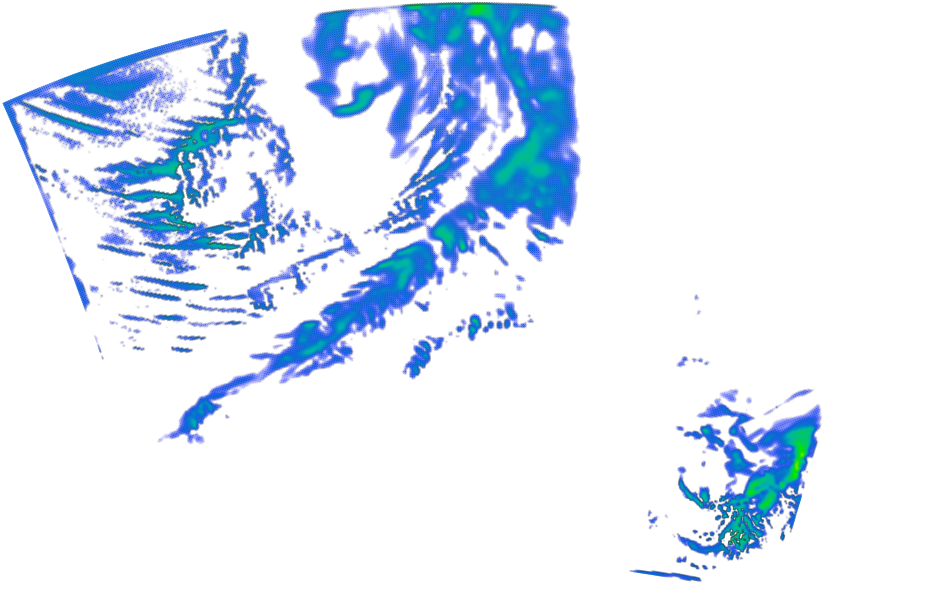
\includegraphics[scale=0.5]{Data/Mdrd_ukazka.png}
	
	\subsubsection{Radar.bourky}
	
	Radar.bourky je datový zdroj který poskytuje data prostřednictvím snímků z radaru, data jsou tedy ve formátu bitmap. Tento datový zdroj je prakticky nepoužitelný, protože poskytuje data pouze v aktuálním čase, respektive v čase pár hodin zpět a pokrávý jen českou republiku. Z toho důvodu se tento zdroj dá využít pouze pro zjištění aktuálního srážek v ČR a blízkém okolí.
	
	\subsubsection{Ukázka API a obsahu}
	
	Ukázka odkazu který vrací bitmapu obsahujícíh data o počasí Evropu v jednom aktuálním čase. Součástí ukázky je i samotná bitmapa \emph{Radar.bourky\_bitmapa} \cite{chmi}.
	
	http://radar.bourky.cz/data/pacz2gmaps.z\_max3d.20201001.1600.0.png
	
	\captionof{figure}{Ukázka snímku z radaru od Radar.bourky}
	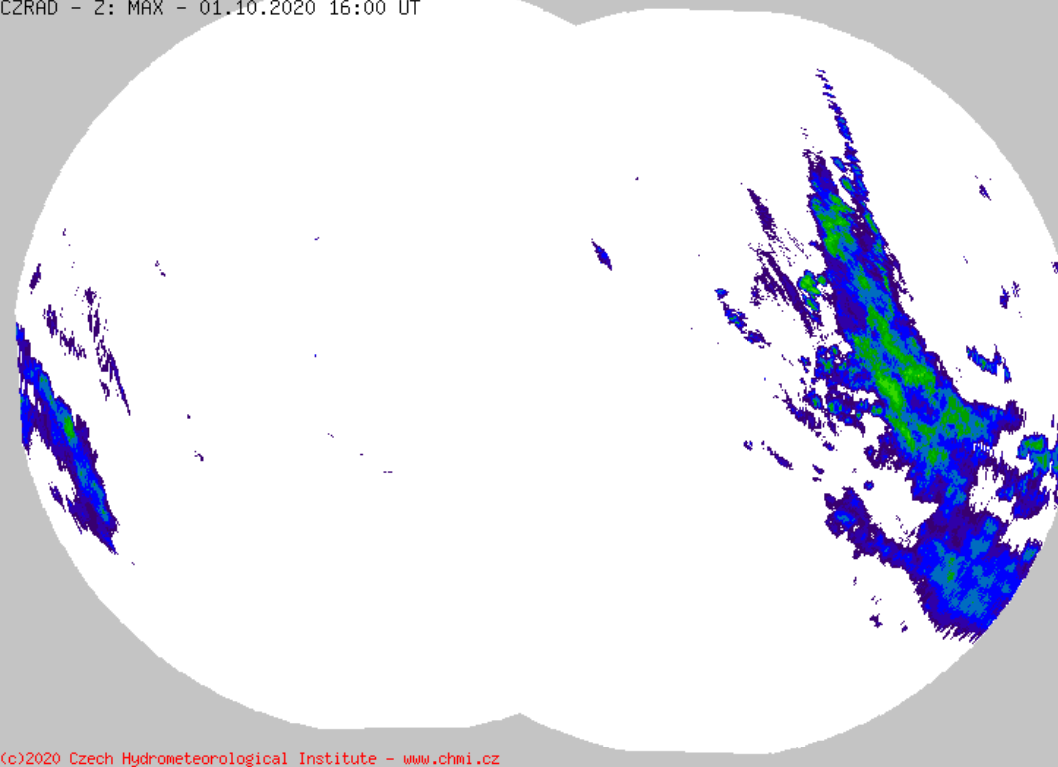
\includegraphics[scale=0.5]{Data/Rb_ukazka.png}
	
	\subsection{Shrnutí použitých zdrojů}
	
	typ = Srážky/Teplot/Tlak/Vlhkost
	
	\captionof{table}{Shrnutí vlastností datových zdrojů}
	\begin{center}
		\begin{tabular} {l r c c l c c c c}
			
			Název & Typ dat & Počet dnů & Hodinový rozdíl & Stažení/min & Plocha & typ \\
			\hline
			Yr.no & XML & 9 & 1 a 6 & & svět & A/A/A/A \\ 
			OpenWeatherMap & JSON & 5 & 3 & 60 & svět & A/A/A/A \\ 
			WeatherUnlocked & JSON & 5 & 3 & 75 & svět & A/A/A/A \\ 
			Medard-online & BMP & 5 & 1 &  & evropa & A/A/N/N \\ 
			Radar.bourky & BMP & 0 & & & ČR & A/N/N/N \\ 
			
		\end{tabular}
	\end{center}
	
	\section{Agregace dat}
	
	Při agregaci dat bylo zapotřebí vyřešit pár otázek. První z nich byla potřeba jednotného výstupního formátu pro různorodá vstupní data, tímto formátem byly zvoleny bitmapy obsahující data o jednom typu počasí, data jsou reprezentována pomocí barev a pokrávají určitou plochu pro určitý čas. Další otázkou bylo jak převádět barvy na číselné hodnoty a hodnoty zpět na barvy, tento problém vyřešilo využití škál. A nakonec jsme potřebovali pokrýt celou bitmapu pokud známe hodnotu počasí pro určíté body, což nám vyřešila triangulace v kombinaci s interpolací.
	
	\subsection{Škála}
	
	Vzhledem k tomu že veškerá data o počasí jsou uložena do bitmap, ve který jsou data reprezentována barvou pixelů vzniká potřeba převádění barvy na číselnou hodnotu a naopak. Práce proto obsahuje metody, které pro určitou barvu vrátí desetinné číslo a pro určité číslo zase barvu.
	
	Nejprve tyto metody obsahovaly desítky podmínek které staticky kontrolovaly zda se jedná o konkrétní barvu, později zda barva patří do určitého rozmezí pro R, G, B složky. Tento přístup ale není vhodný, protože při potřebě změnit barvy pro určitá desetinná čísla vznikala nutnost přepsat hodnoty barev pro všechny metody ve veškerých podmínkách.
	
	Finálním řešením se stalo využití škál, škály jsou obrázky široké přesné tolik pixelů kolik hodnot uchovávají, kde každý pixel obsahuje unikátní barvu a reprezentuje jednu konkrétní číselnou hodnotu kterou daná barva reprezentuje. Výška škály může být pouze 1 pixel. Výhoudou škál je, že změna barev reprezentujících hodnoty případně změna rozsahu uchovávanách hodnot se vyměnit pouze pomocí použití nové škály která bude opět orientovaná na šířku. Další z výhod je že metody které vrací hodnotu z barvy nemusí obsahovat desítky podmínek a stačí pouze vrátit hodnotu uloženou pro pixel. V programu jsou barvy ze škály uložený do slovníku, kde klíč reprezentuje barva a hodnotu desetinné číslo. Pro určení čísla z barvy stačí vypočítat index na kterém barva leží a tuto barvu vrátit.
	
	\subsection{Triangulace}
	
	Při vytváření bitmap dochází k určování hodnot počasí (teplota, srážky atp.) pro konkrétní zeměpisné souřadnice, které jsou následně převedeny na pixely bitmapy. Zjišťovat hodnotu pro každý jednotlivý pixel by bylo velice časově náročné, a protože můžeme předpokládat že v okolí pixelu budou obdobné hodnoty jako na pixelu samotné stačí nám určit hodnoty pouze pro určité množství pixelů rozložených správně po bitmapě. Následně je potřeba tyto pixely nějakým způsobem propojit, zde nám problém řeší využité triangulace.
	
	V práci se využívá S-hull Algoritmus pro triangulaci. Konkrétně Phil Atkinova implementace pro C\#. Algoritmus nám množinu bodů, v našem případě pixelů, rozdělí na trojuhelníky. Respektive nám pro každý vrchol řekne s kterými vrcholi je spojen hranou, čímž nám vznikne síť trojuhelníků pokrývající většinu bitmapy.
	
	%\vfill
	
	S-hull algoritmus slouží pro vytvoření Delaunayovi triangulace z množiny 2D bodů s časovou složitostí $O(n  log(n))$. Algoritmus využívá radiálního šíření, které se postupně vytváří z radiálně seřezené množiny 2D bodů, a je zakončen převracením trojuhelníků čímž se získá Delaunayova trinaguzlace. Tento algoritmus ve srovnásí s Q-hull algoritmem dosahuje přibližně polovičního času při vytváření triangulace pro náhodně generované množiny 2D bodů. S-hull je pro množinu unikátních 2D bodů $x_i$ implementován následovně:
	\begin{enumerate}
		\item Vybere počáteční bod $x_0$ z množiny bodů $x_i$.
		\item Seřadí body dle vzdálenosti od tohoto bodu $|x_i - x_0|^2$.
		\item Nalezne bod $x_j$, který je k bodu $x_0$ nejblíž.
		\item Nalezne bod $x_k$, který vytvoří nejmenší kružnici opsanou s body $x_0$ a $x_j$ současně i zaznamená střed kružnice opsané $C$.
		\item Seřadí body $x_0$, $x_j$, $x_k$ pro získání pravorukého systému, tohle je počateční prvek pro convex hull.
		\item Přetřídí zbývající body na základě vzdálenosi bodů od středu kružnice opsané $|x_i - C|^2$ pro získání bodů $s_i$.
		\item Postupně se přidávají body $s_i$ do rostoucího 2D convex hull který je závislý na trojuhelníku vytvořeném z bodů $x_0$, $x_j$, $x_k$. Následné jsou přidány zkosené hrany pro 2D-hull, které jsou bodu viditelné z nově vytvořených trojuhelníků.
		\item Vzájemně se nepřekrývající triangulace pro množinu bodů je nyní vytvořena. Tato metoda je velice rychlá mezi způsoby vytváření 2D triangulace.
		\item Sousední páry trojuhelníků této triangulace musí být \uv{převráceny} aby došlo k vytvoření Delaunayovi triangulace z počáteční nepřekrývající se triangulace.
	\end{enumerate}
	
	\subsection{Interpolace}
	
	Bitmapa je pokryta sítí trojuhelníků kde známe hodnotu každého vrcholu. Nyní vzniká potřeba každý trojuhelník vyplnit barvamy, které reprezentují hodnotu pixelů uvnitř trojuhelníku. Tuto práci řeší využití interpolace, nebole výpočet hodnoty uvnitř objektu na základě vzdálenosti od vrcholů.
	
	Pro výpočet interpolace postačí jednoduchý vzorec, který na základě hodnot vrcholů trojuhelníku a vzdálenosti od nich pro zjišťovanáý bod určí jakou hodnotu sám zjišťovaný bod má.
	
	%\vspace{10mm}
	
	V prvním kroku výpočtu je zapotřebí spočítat vzdálenost $Distance$ zjišťovaného bodu $P$ od všech tří vrcholů trojuhelníku $V_1$, $V_2$, $V_3$. 
	
	\[Distance_{v1} =\sqrt{(X_{v1}-P_x)^2+(Y_{v1}-P_y)^2}\]
	\[Distance_{v2} =\sqrt{(X_{v2}-P_x)^2+(Y_{v2}-P_y)^2}\]
	\[Distance_{v3} =\sqrt{(X_{v3}-P_x)^2+(Y_{v3}-P_y)^2}\]
	
	Následně se určí váha každého vrcholu $W$, neboli inverní hodnota jeho vzdálenosti od zjišťovaného bodu.
	
	\[W_{v1} =\frac{1}{Distance_{v1}}\]
	\[W_{v2} =\frac{1}{Distance_{v2}}\]
	\[W_{v3} =\frac{1}{Distance_{v3}}\]
	
	Ve finálníčásti výpočtu se určí hodnota našeho zjišťovaného bodu $Value_p$, která je úměrná podílu součtu součíná váh a hodnot jednotlivých vrcholů trojuhelníku se seoučtem jendotlivých váh.
	
	\[Value_p = \frac{W_{v1}Value_{v1} + W_{v2}Value_{v2} + W_{v3}Value_{v3}}{W_{v1} + W_{v2} + W_{v3}} \]
	
	
	\section{Distribuce dat}
	
	Shromážděné a zprůměrované předpovědi počasí je potřeba nějakým způsobem dodávat klientovi. Tuto úlohu nám splní webová služba, která pro různé dotazy ve formě url API vrací agregovaná data o počasí v požadovaných formátech. Služba se implementovala jako MVC aplikace pro C\# a využívá pro svou práci knihovnu pro agregaci dat z předešlé sekce. Vzhledem k tomu že jsou data o počasí uložená do bitmap, lze informace o počasí poskytovat i bez připojení k internetu, musíme však mít pro dané časy bitmapy dopředu vytvořené. Služba volá požadavek o vytvoření bitmap vždy při spuštění a následně každou další hodnu běhu, jednotlivé datové zdroje si následně zjistí kdy byly bitmapy naposledy vytvořený a pokud již uplynul minimální čas dojde k vytváření bitmap nových, tento čas se může u každého datového zdroje lišit.
	
	\subsection{API}
	
	Při práci se službou se využívá vytvořeného API které pro správně zadané vstupní parametry vrácí požadovanou předpověď. Webová služba vrací data ve třech formátech xml, json a bitmapa. Nakonec je možné získat jednotlivé škály, které služba využívá pro správu dat o počasí v bitmapách.
	
	\subsubsection{Bitmap předpověď}
	
	Tato předpověď se získává požadavkem bmp a vždy vrací bitmapu o rozměrech 728x528 pixelů pokrývající určitou plochu. Plocha je vymezená body zeměpisných souřadnic, konkrétně levým horním $p1$ a pravým dolním $p2$ rohem. Pokud nedojde k zadání těchto bodů je bitmapa určenapro Českou republiku. Při určování této předpovědi je zapotřebí rovněž i čas pro který se má předpověď určitě $time$, tento čas musí být ve formátu ISO 8601 a pokud není zadán nebo je místo něj vyplněna hodnota 0 určí se předpověď pro aktuální čas požadavku předpovědi. Následně je potře zadat typ předpovědi $type$, který má bitmapa reprezentovat tyto typy jsou 2 typ prec reprezentuje srážky v mm a typ temp teplotu ve stupních Celsia. Nakonec se zadávají datové zdroje $loaders$, takzvané loadery, ze kterých má služba získávat data. Je potřeba zadat zkratky loaderů oddělené čárkami pro každý loader který má služba využít pokud není zadán žádný loader použijí se všechny dostupné současně.
	\\\\
	adresaserveru/bmp?type=\{typ\}\&time=\{čas\}\&loaders=\{datové zdroje\}\&p1=\{bod1\}\&p2=\{bod2\}
	
	\captionof{table}{Parametry bitmap předpovědí}
	\begin{center}
		\begin{tabular}{c c p{13cm}}
			Název & Povinnost & Význam \\
			\midrule
			type & ANO & Typ předpovědi, určuje druh vykreslených informací. Například typ $prec$ reprezentuje srážky v milimetech a typ $temp$ teplotu ve stupních Celsia.\\ 
   			time & NE & Čas předpovědi, pokud je zadán musí být ve formátu ISO 8601. Pokud zadán není nebo je zadána hodnota 0  provede se předpověď pro aktuální čas.\\ 
   			loaders & NE & Datové zdroje které se mají použít. Výběr datových zdroju se provede zadáním zkratek jednotlivých zdrojů oddělených čárkami. Pokud je parametr prázdný použijí se veškeré datové zdroje služby. \\ 
   			p1 & NE & Levý horní roh vymezující plochu bitmapy. Bod reprezentuje zeměpisné údaje v pořadí zeměpisná šířka a délka (latitude a longitude), údaje jsou odděleny čárkou. Pro oddělení celé a desetinné části souřadnice se používá tečka. Pokud bod $p1$ a $p1$ není zadán, bitmapa se vykreslí pro celou možnou plochu.\\
   			p2 & NE & Pravý dolní roh vymezující plochu bitmapy. Bod reprezentuje zeměpisné údaje v pořadí zeměpisná šířka a délka (latitude a longitude), údaje jsou odděleny čárkou. Pro oddělení celé a desetinné části souřadnice se používá tečka. Pokud bod $p1$ a $p1$ není zadán, bitmapa se vykreslí pro celou možnou plochu.\\
		\end{tabular}
	\end{center}
	
	Příklady požadavků:
	\begin{itemize}
		\item Požadujeme bitmapu s daty o teplotě pro aktuální čas, která pokrývající celou možnou plochu a využívá veškeré datové zdroje.
		\begin{itemize}
			\item adresaserveru/bmp?type=temp
		\end{itemize}
		\item Požadujeme bitmapu s daty o srážkách pro 26. 5. 2021 18:30, která pokrývající celou možnou plochu a využívá datové zdroje od služeb OpenWeatherMap a Yr.No.
		\begin{itemize}
			\item adresaserveru/bmp?type=prec\&time=2021-05-26T18:30:00\&loaders=owm,yrno
		\end{itemize}
		\item Požadujeme bitmapu s daty o srážkách pro aktuální čas, která pokrývající město Olomouc a využívá datový zdroj od služby Medard-Online.
		\begin{itemize}
			\item adresaserveru/bmp?type=prec\&p1=49.621559,17.1507294\&p2=49.5211889,17.4213141\&loaders=mdrd
		\end{itemize}
	\end{itemize}

	\subsubsection{XML a JSON předpověď}
	
	Tento požadavek nám dovoluje získat data o počasí pro určitý bod v zadaném čase, případně lze určit data o počasí pro více časů za sebou s konstantním hodinovým rozdílem. Při získávání XML nebo JSON dat potřebujeme zadat stejně jako u bitmap předpovědí zadat parametr požadovaného času $time$ a datové zdroje které tento čas zpracovávají $loaders$. Dále musíme zadat požadovaný typ dat XML/JSON $data$ a zeměpisný bod pro který chceme počasí určit, bod se skládá z parametrů $lon$ a $lat$. Pro získání více časových oken v jedné předpovědi musíme přidat parametr reprezentující počet předpovědí $numOfFcs$ a hodinový rozdíl mezi těmito předpověďmi $hourDif$.
	\\\\
	adresaserveru/{data}?time={čas}\&lat={zeměpisná\_šířka}\&lon={zeměpisní\_délka}\&loaders={datové\_zdroje}
	
	adresaserveru/{data}?time={čas}\&numOfFcs={počet\_předpovědí}\&hourDif={hodinový\_rozdíl\_mezi\_předpověďmi}\&lat={zeměpisná\_šířka}\&lon={zeměpisní\_délka}\&loaders={datové\_zdroje}
	
	\captionof{table}{Parametry xml/json předpovědí}
	\begin{center}
		\begin{tabular}{c c p{13cm}}
			Název & Povinnost & Význam \\
			\midrule
			data & ANO & Formát v jakém mají být data o počasí zpracována. Rozlišujeme dva typy a to $xml$ a $json$.\\
			lon & ANO & Longitude, parametr reprezentující zeměpisnou délku požadované souřadnice. Desetinná a celá část souřadnice jsou odděleny tečkou.\\
			lat & ANO & Latitude, parametr reprezentující zeměpisnou šířku požadované souřadnice. Desetinná a celá část souřadnice jsou odděleny tečkou.\\
			time & NE & Čas předpovědi, pokud je zadán musí být ve formátu ISO 8601. Pokud zadán není nebo je zadána hodnota 0  provede se předpověď pro aktuální čas.\\ 
			loaders & NE & Datové zdroje které se mají použít. Výběr datových zdroju se provede zadáním zkratek jednotlivých zdrojů oddělených čárkami. Pokud je parametr prázdný použijí se veškeré datové zdroje služby. \\
			numOfFcs & NE & Počet časových oken které má předpověď obsahovat. Pokud není tento parametr zadán, v předpovědi bude právě jedno časové okno pro zadaný čas.\\
			hourDif & NE & Hodinový rozdíl mezi jednotlivými časovými okny v předpovědi. Pokud není tento parametr zadán, v předpovědi bude právě jedno časové okno pro zadaný čas.\\
		\end{tabular}
	\end{center}

	Příklady požadavků:
	\begin{itemize}
		\item Požadujeme předpověď o počasí pro aktuální čas v Ostravě zpracovanou všemi datovými zdroji ve formátu xml.
		\begin{itemize}
			\item adresaserveru/xml?lon=18.262524\&lat=49.820923
	   \end{itemize}	
		\item Požadujeme předpověď o počasí pro datum a čas 14.03.2021 18:35 v Ostravě zpracovanou všemi datovými zdroji ve formátu json.
		\begin{itemize}
			\item adresaserveru/json?lon=18.262524\&lat=49.820923\&time=2021-03-14T18:35:00
		\end{itemize}
		\item Požadujeme předpověď o počasí pro datum a čas 14.03.2021 18:35 v Ostravě zpracovanou datovými zdroji OpenWeatherMap a WeatherUnlocked ve formátu xml.
		\begin{itemize}
			\item adresaserveru/xml?lon=18.262524\&lat=49.820923\&time=2021-03-14T18:35:00\&loaders=owm,weun
		\end{itemize}
		\item Požadujeme předpověď o počasí v Ostravě pro 5 časových oken s 3 hodinovými rozestupy počínaje aktuálním časem.
		\begin{itemize}
			\item adresaserveru/json?lon=18.262524\&lat=49.820923\&time=2021-03-14T18:35:00\&numOfFcs=5\&hourDif=3
		\end{itemize}
	\end{itemize}
	
	\subsubsection{Využívané škály}
	
	Služba nám umožňuje stažení jednotlivých škál, které používá při zpracovávání bitmap s daty o počasí. Stačí znát zkratku typu počasí a služba nám vrátí využívanou škálu.
	
	Příklady požadavků:
	\begin{itemize}
		\item Požadujeme škálu pro teploty.
		\begin{itemize}
			\item adresaserveru/scale?type=temp
		\end{itemize}
		\item Požadujeme škálu pro srážky.
		\begin{itemize}
			\item adresaserveru/scale?type=prec
		\end{itemize}
	\end{itemize}
	
	\subsubsection{Zkratky typů počasí}
	
	Zkratky pro jednotlivé typy předpovědí které se využívají v parametru type.
	
	\captionof{table}{Zkratky typů předpovědí}
	\begin{center}
		\begin{tabular}{c c c}
			Typ počasí & Jednotka & Zkratka pro API\\
			\midrule
			Srážky & mm & prec \\
			Teplota & °C & temp \\
			Tlak & hPa & pres \\
			Vlhkost & \% & humi \\
		\end{tabular}
	\end{center}
	
	\subsubsection{Zkratky datových zdrojů}
	
	Zkratky pro jednotlivé datové zdroje které se využívají v parametru loaders. Při použití více zkratek za sebou oddělených čárkou dojde k použití více zdrojů současně.
	
	\captionof{table}{Zkratky datových zdrojů}
	\begin{center}
		\begin{tabular}{c c}
			Celý název datového zdroje & Zkratka pro API\\
			\midrule
			Radar.bourky & rb \\
			Medard-online & mdrd \\
			OpenWeatherMap & owm \\
			Yr.no & yrno \\
			WeatherUnlocked & weun \\
		\end{tabular}
	\end{center}
	
	\subsection{Chyba při zpracování dat}
	
	Při požadavku o dodání dat může dojít k chybě, nejčastěji při chybném zadání parametrů v API, případně i při požadování dat pro čas který ještě bitmapami není zpracován. Pokud tato situace nastane služba místo požadovanách dat vráti json text obsahující jediný parametr $message$ obsahující informace proč k pádu došlo a jak parametry upravit aby se chyba neopakovala a bylo možné nějaké informace o počasí získat.
	
	\section{Vizualizace dat}
	
	\section{Závěr}
	
	\printbibliography[title={Literatura}, heading=bibintoc]

	
\end{document}
